\chapter{Keystone Configuration}
\par based on the documentation, Keystone is an OpenStack service that provides API client authentication, service discovery, and distributed multi-tenant authorization by implementing OpenStack’s Identity API; which mean that keystone is the service that will be used as the authentication service and also will provide each user the services that he can use. And this section is dedicated to Keystone installation and configuration.
\begin{spacing}{1.2}
%note en bas de page
\section{Add a User and Database on MariaDB for Keystone}

\par In this section, we will install and configure OpenStack Identity Service (Keystone). We
are going to connect to MariaDb so that we can add a user and a database
for Keystone. 
\\
\begin{figure}[!htb] 
\begin{center} 
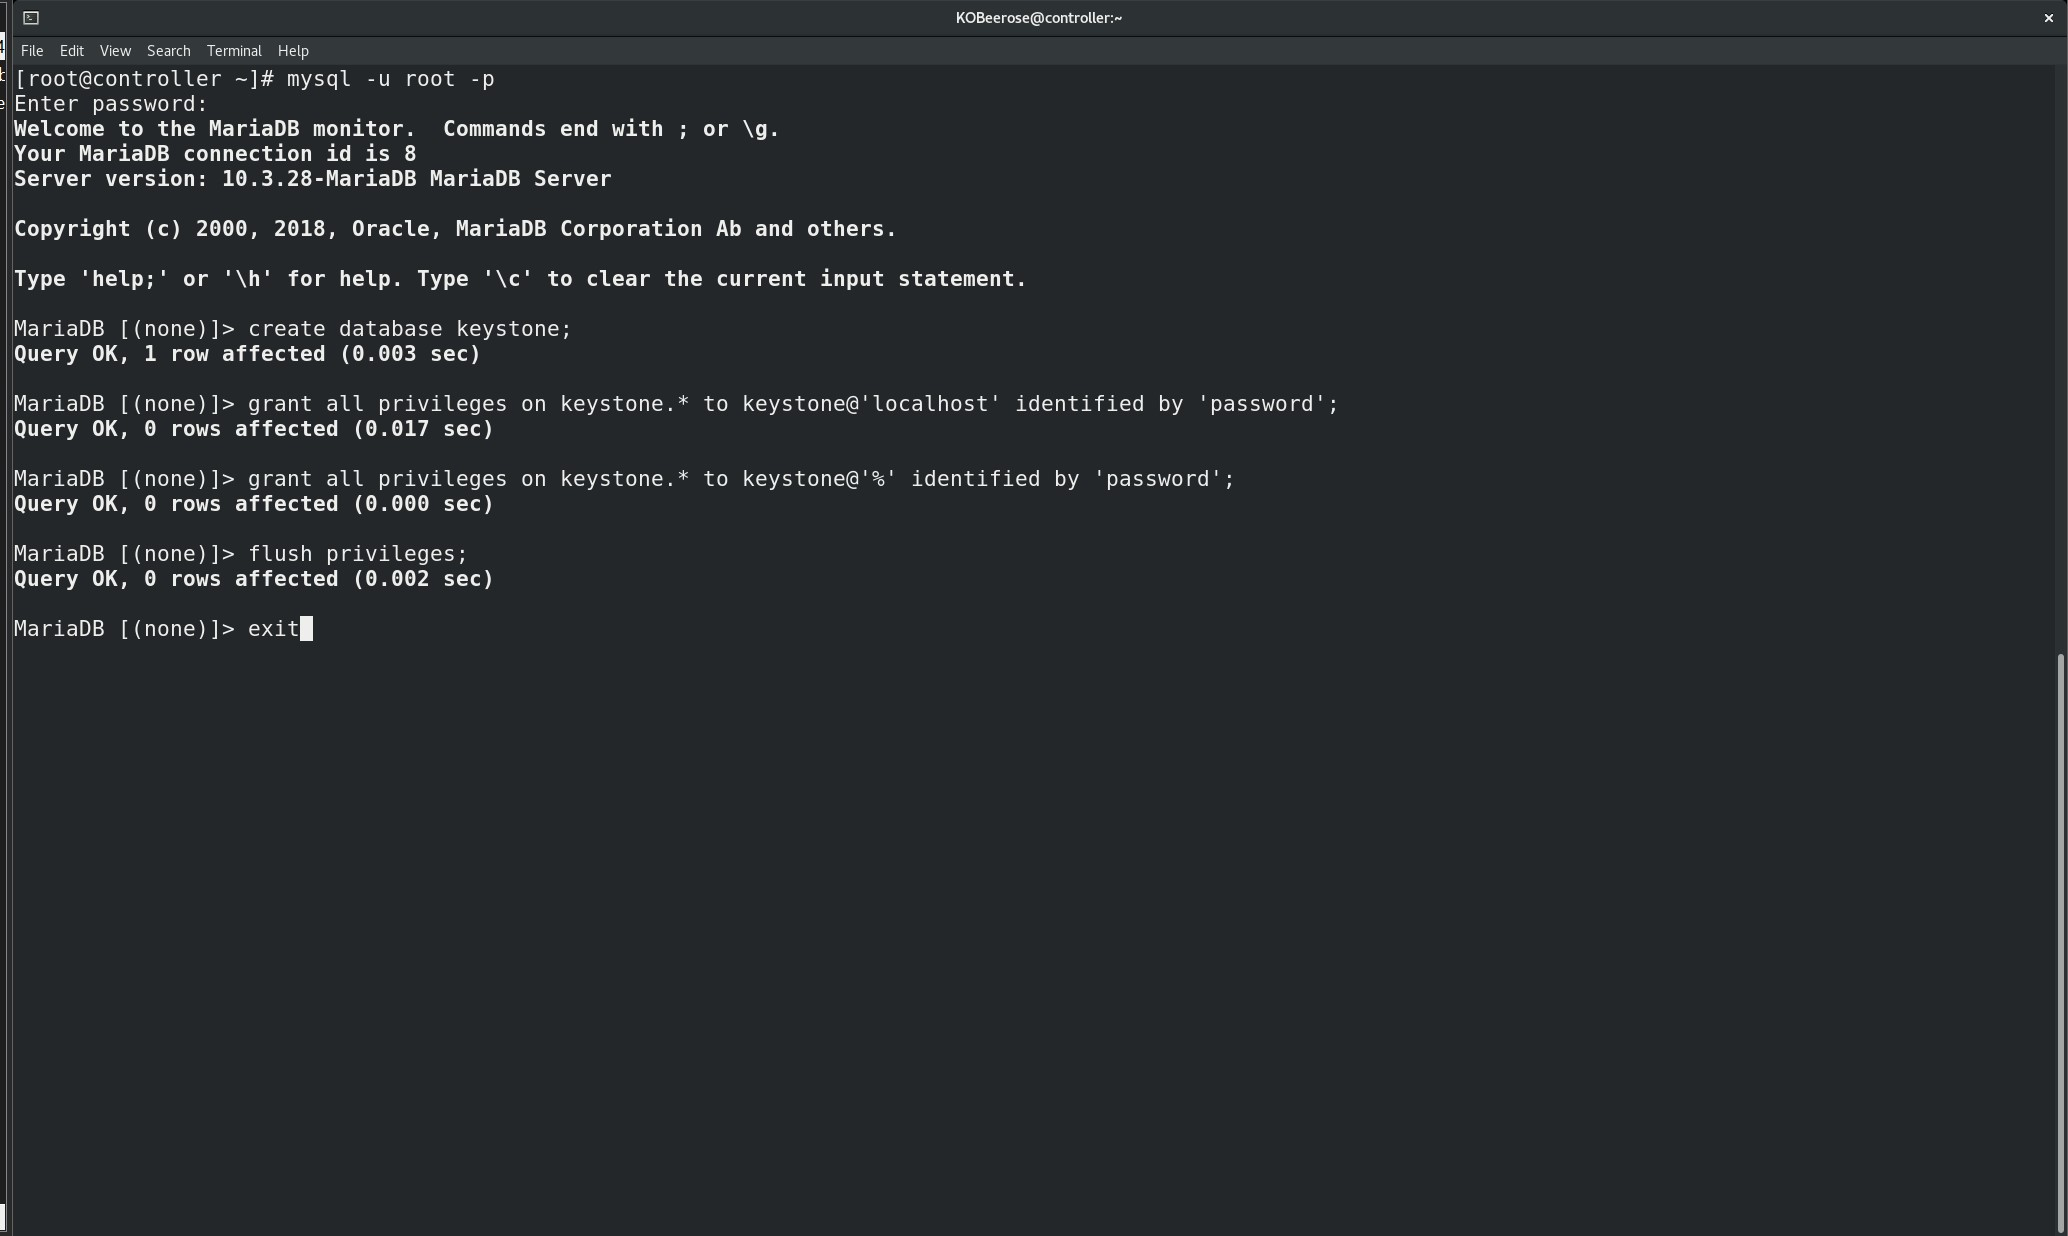
\includegraphics[width=1\linewidth]{Cloud/Configure Keystone #1/Add a user and DB for Keystone} 
\end{center} 
\caption{Add a user and DB for Keystone} 
\end{figure}  \FloatBarrier
\\


\section{Installing Keystone}

\par To install Keystone, we need to install many packages as shown in the
figure below: 
\\
\begin{figure}[!htb] 
\begin{center} 
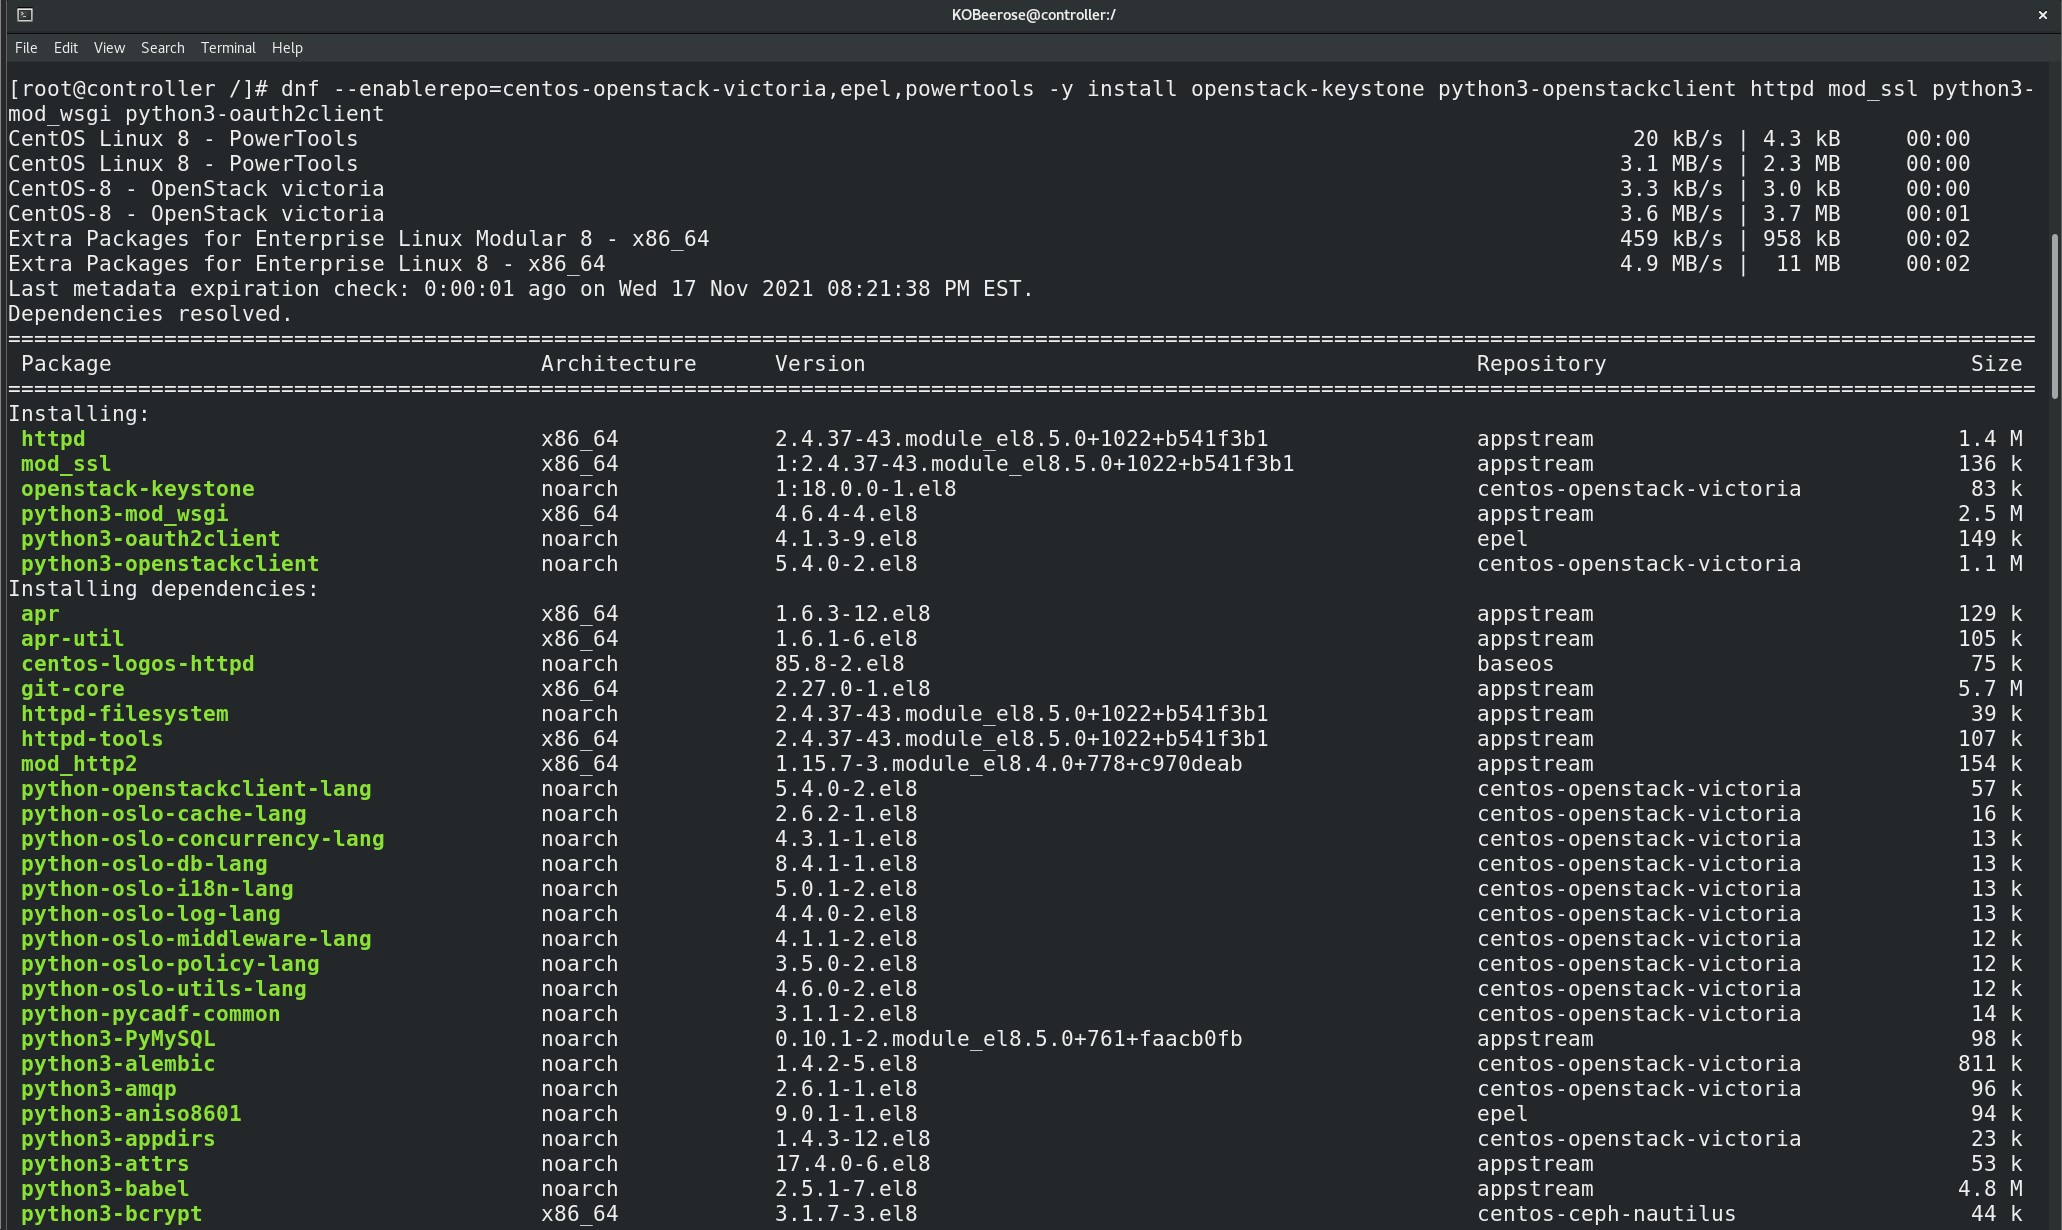
\includegraphics[width=1\linewidth]{Cloud/Configure Keystone #1/Installing EPEL, powertools} 
\end{center} 
\caption{Installing EPEL, powertools} 
\end{figure}  \FloatBarrier
\\


\section{Configure Keystone.}

\par To configure Keystone, we will specify the Memcache server, specify the information
MariaDB connection and comment on the Provider Fernet .\\

\\
\begin{figure}[!htb] 
\begin{center} 
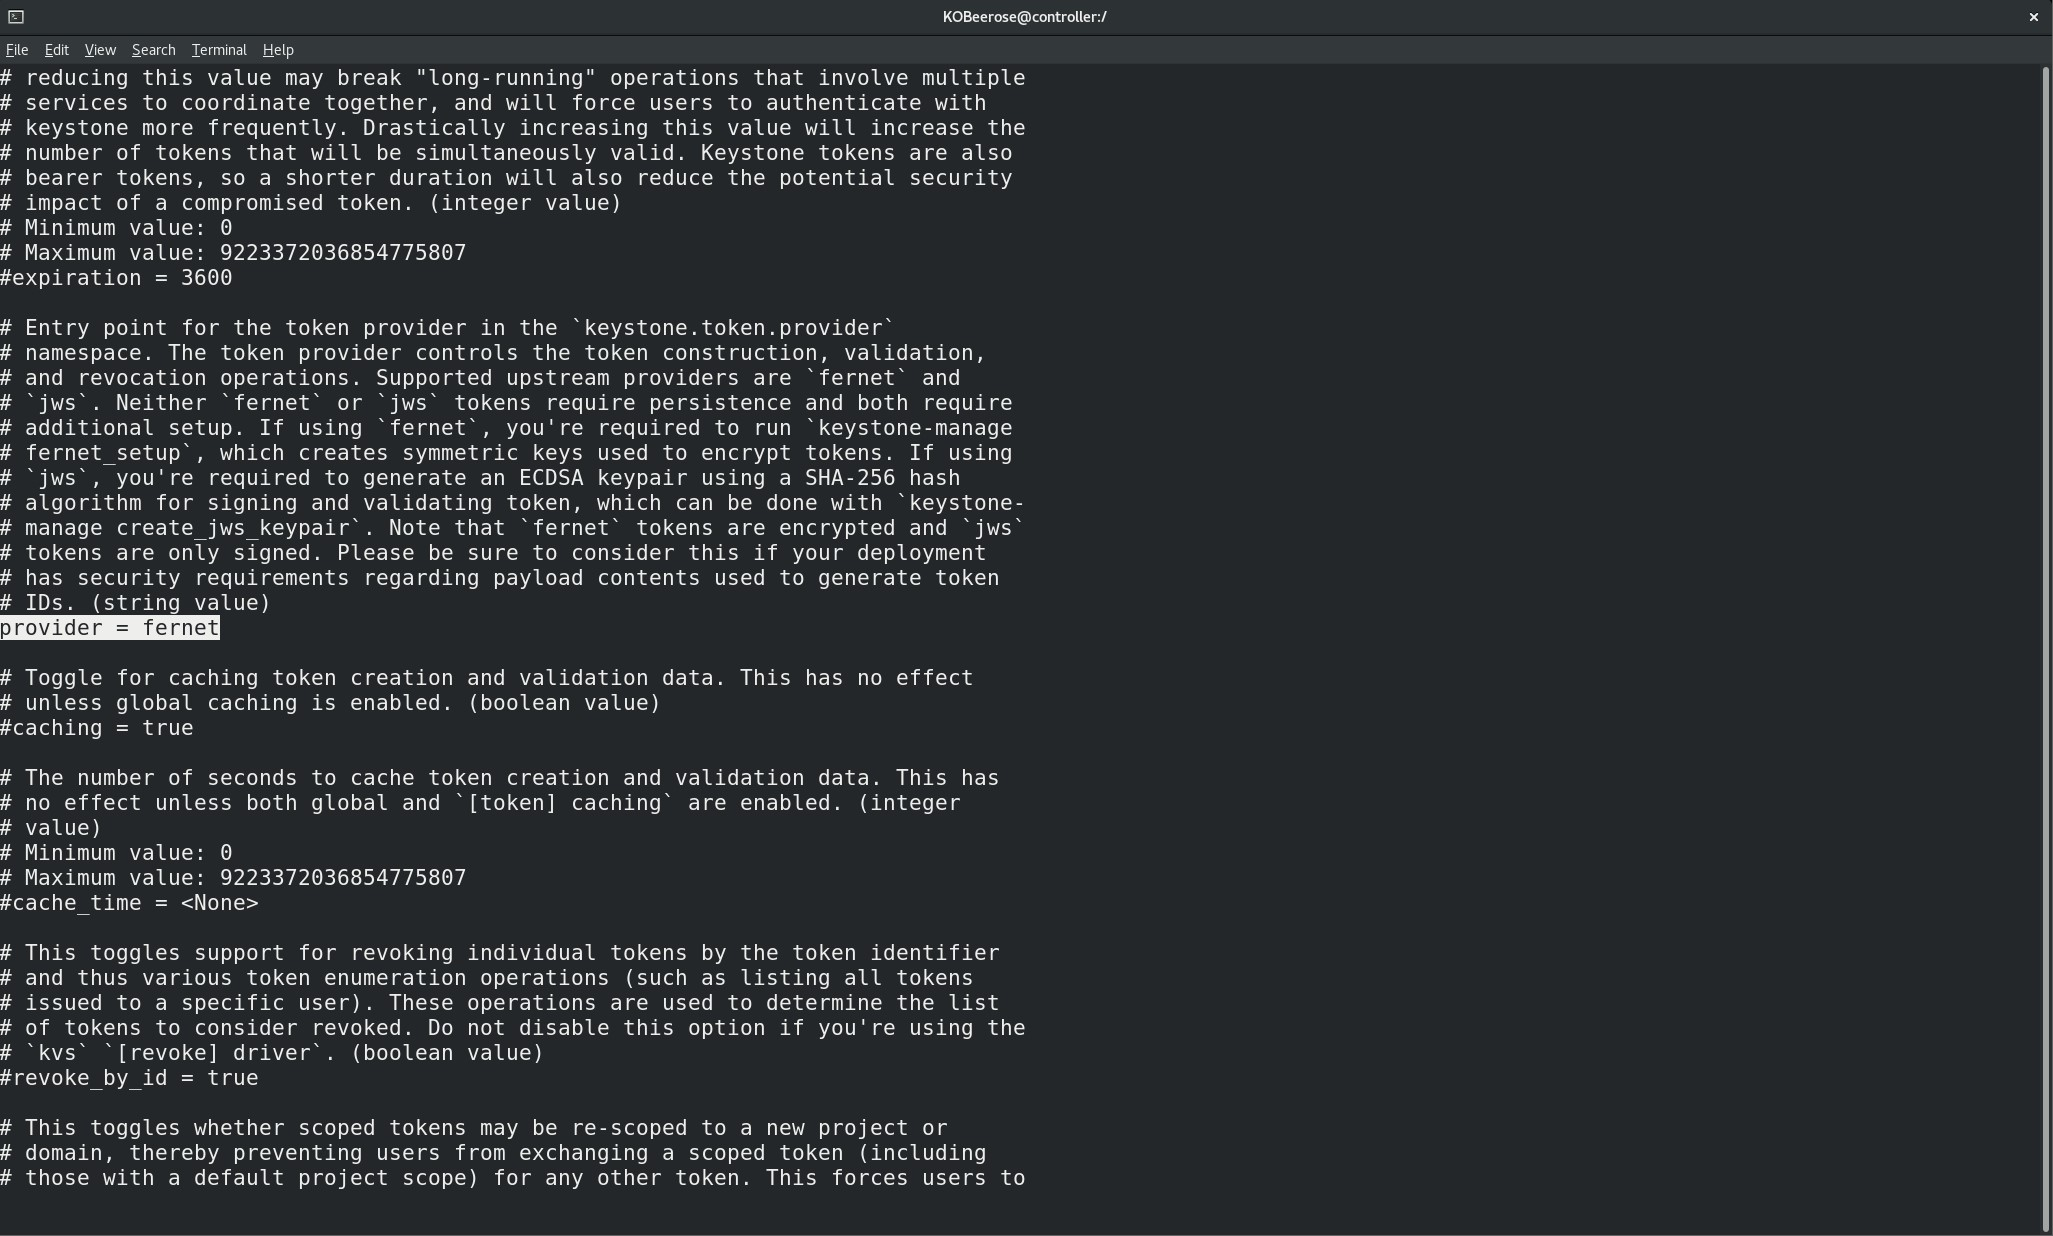
\includegraphics[width=1\linewidth]{Cloud/Configure Keystone #1/keystone.conf file} 
\end{center} 
\caption{keystone.conf file} 
\end{figure}  \FloatBarrier
\\
\par After having synchronized Keystone, we will initialize the keys, define Keystone Host and
run the keystone-manage bootstrap command to create a user, project, and role, and
assign roles. By default, the names of these new resources will be called admin. 
\\
\begin{figure}[!htb] 
\begin{center} 
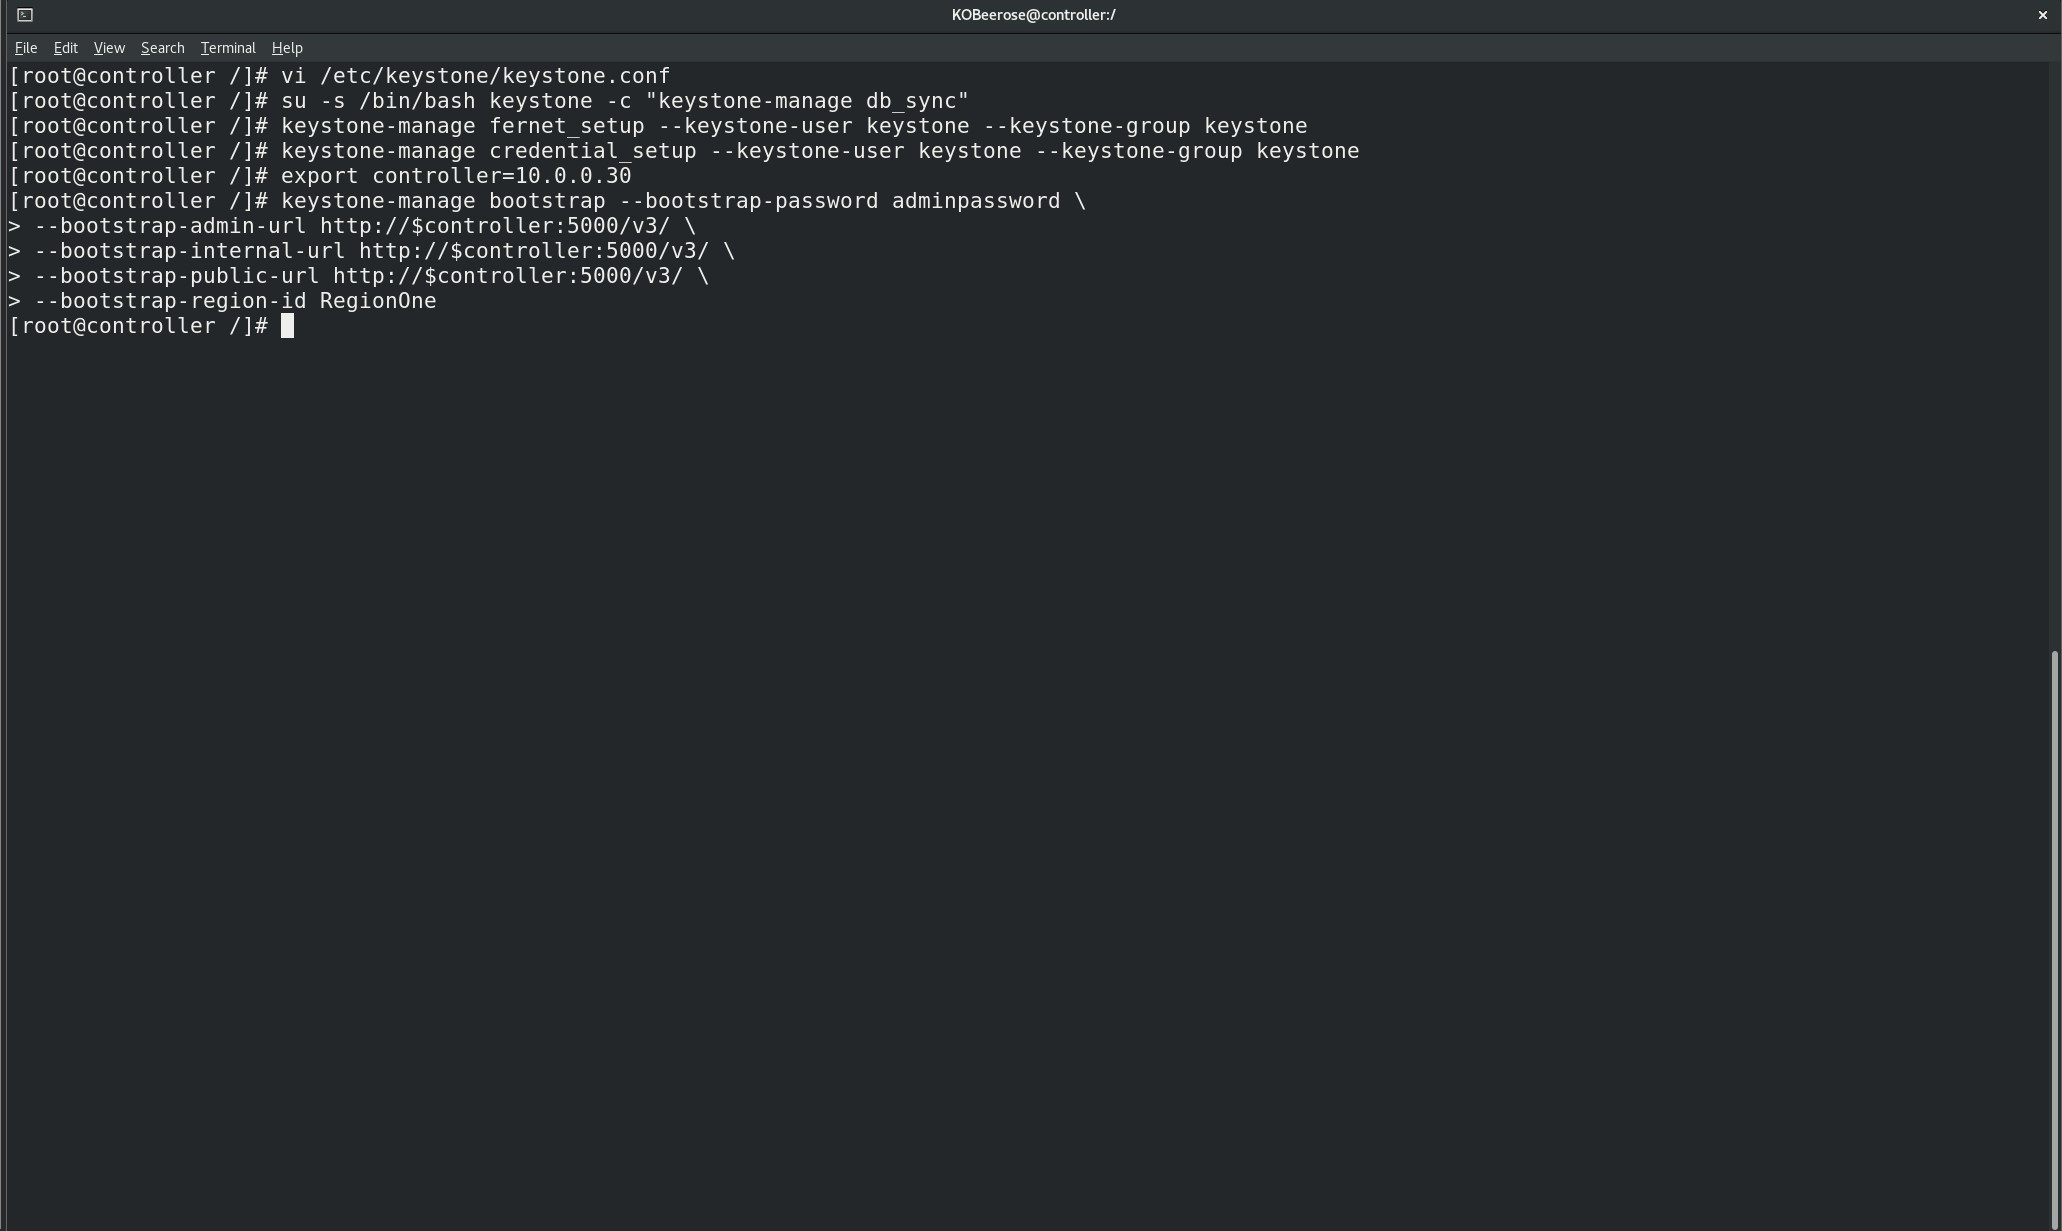
\includegraphics[width=1\linewidth]{Cloud/Configure Keystone #1/Configure Keystone} 
\end{center} 
\caption{Configure Keystone} 
\end{figure}  \FloatBarrier
\\
\section{keystone-httpd config}
\par 
As always, we need to change the boolean parameters of selinux and change the policy by creating a new module keystone-httpd.te to compile as shown below
\\
\begin{figure}[!htb] 
\begin{center} 
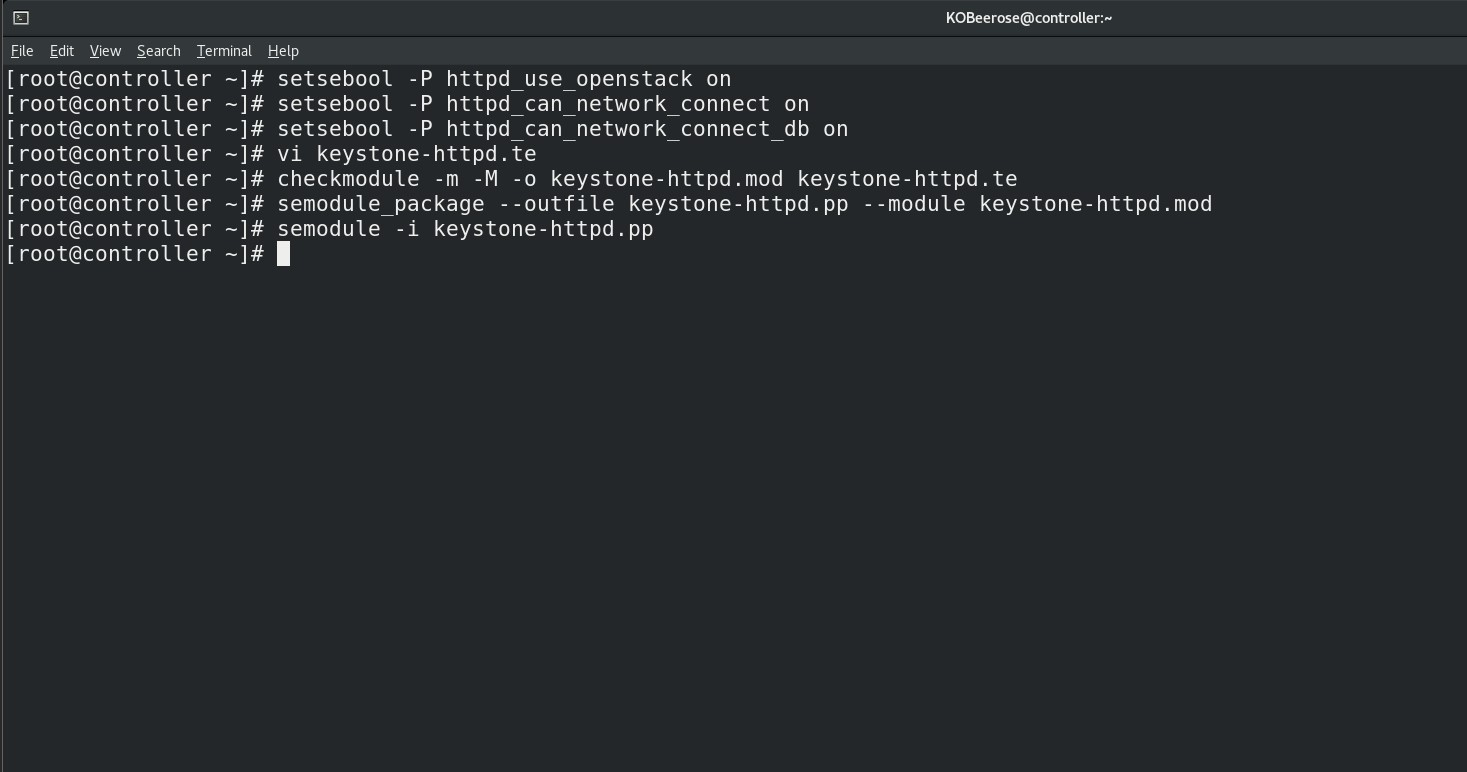
\includegraphics[width=1\linewidth]{Cloud/Configure Keystone #1/keystone-httpd config} 
\end{center} 
\caption{keystone-httpd config} 
\end{figure}  \FloatBarrier
\\
\section{Starting Apache httpd}
\par 
First step is allowing the port 5000 service and reloading the firewall.
\\
\begin{figure}[!htb] 
\begin{center} 
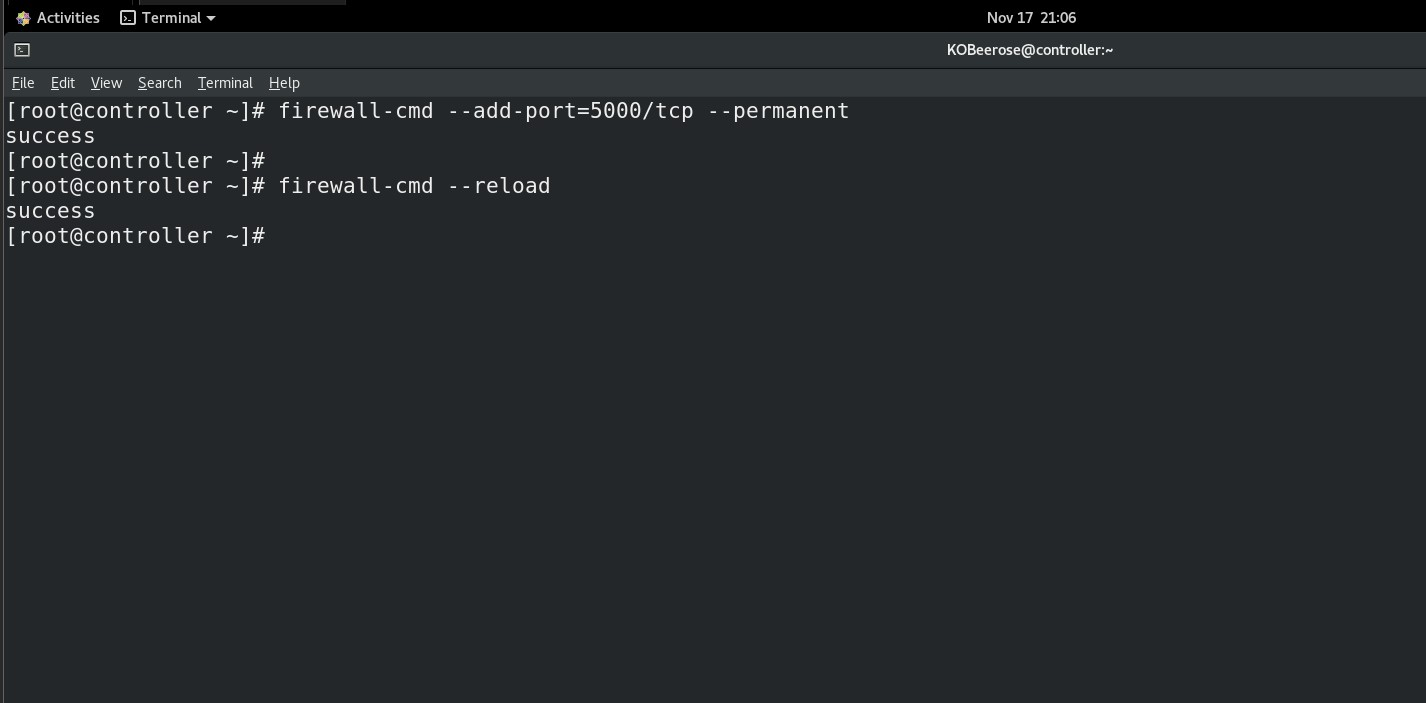
\includegraphics[width=1\linewidth]{Cloud/Configure Keystone #1/Allowing 5000 port} 
\end{center} 
\caption{Allowing 5000 port} 
\end{figure}  \FloatBarrier
\\
\par 
Once everything is configured, we will modify the /etc/httpd/conf/httpd.conf file to set the server name, then start Apache httpd. 
\\
\begin{figure}[!htb] 
\begin{center} 
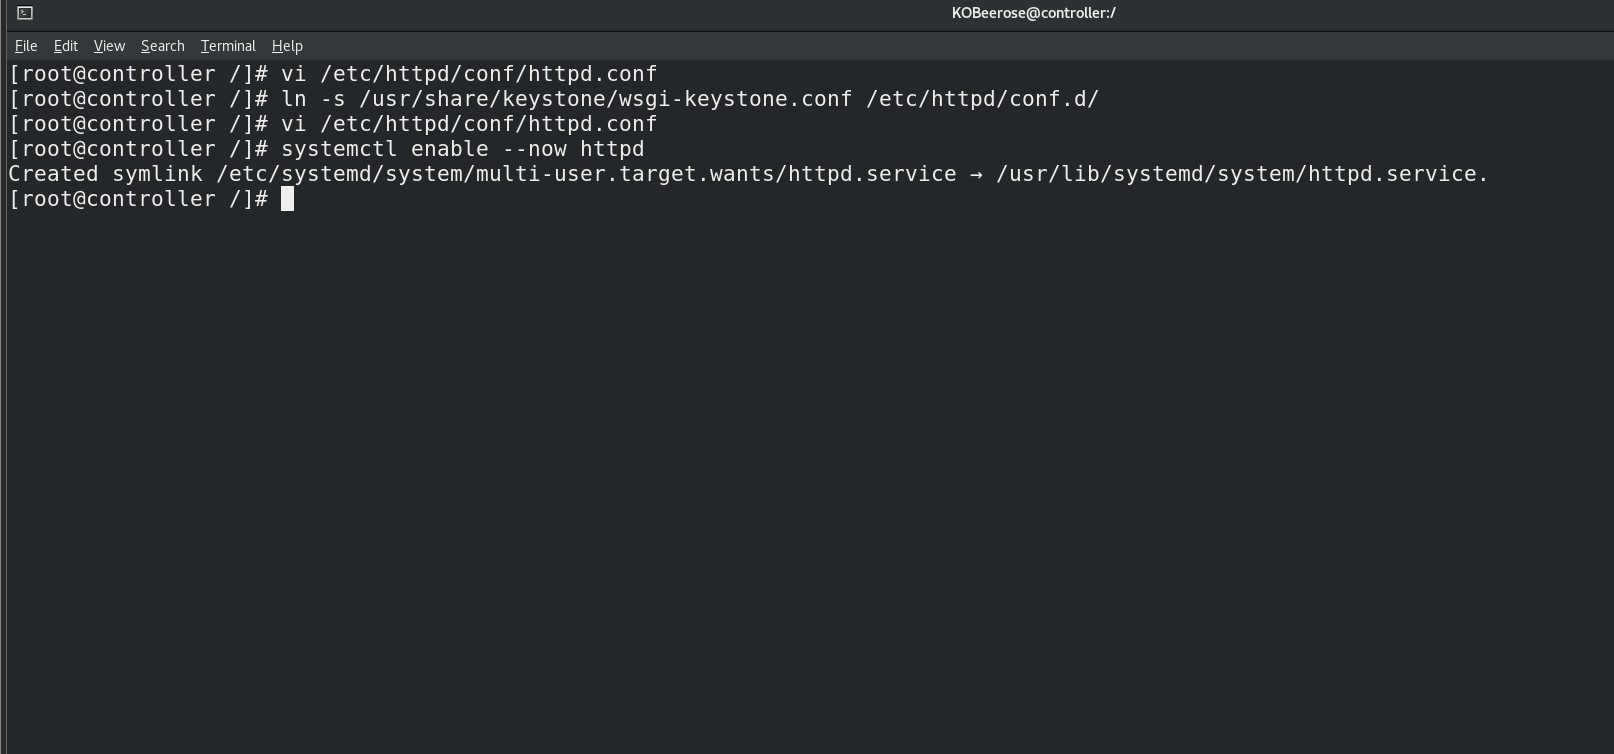
\includegraphics[width=1\linewidth]{Cloud/Configure Keystone #1/Apache httpd} 
\end{center} 
\caption{Apache httpd} 
\end{figure}  \FloatBarrier
\\
\section{Creating and Load environment variables file}

\par One more step before creating keystone projects, we are going to export some environment variables written in the  / keystonerc file as shown below: 
\begin{figure}[!htb] 
\begin{center} 
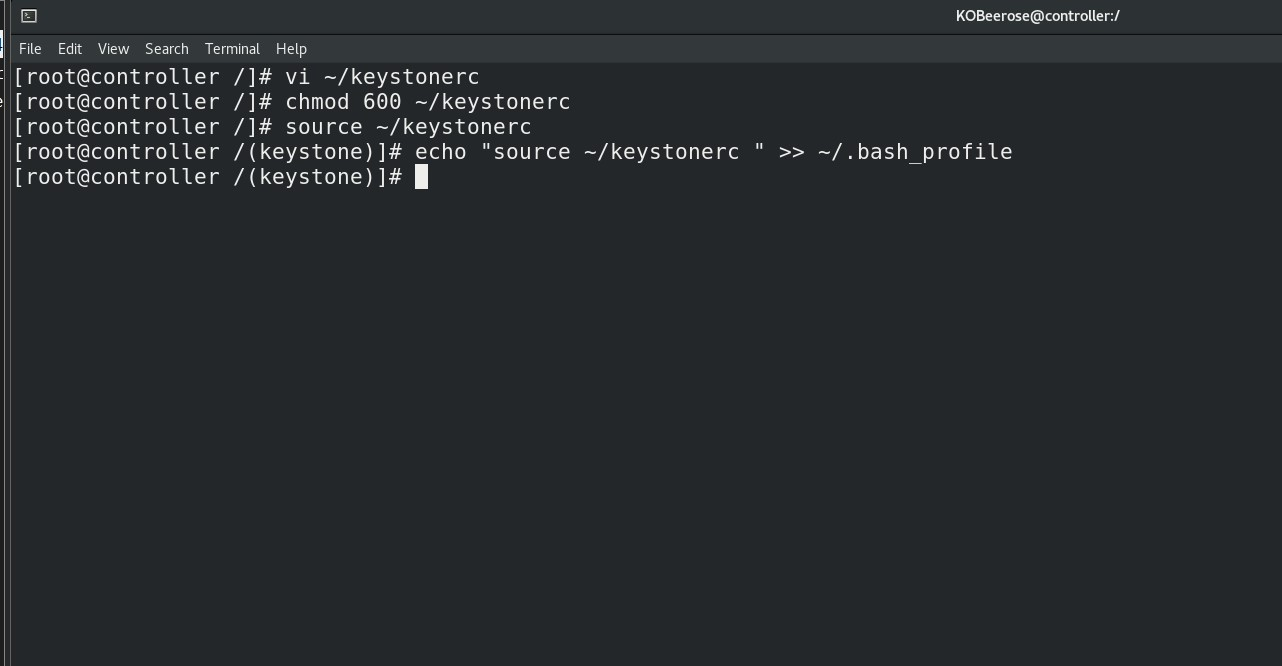
\includegraphics[width=0.94\linewidth]{Cloud/Configure Keystone #2/Creating env var file} 
\end{center} 
\caption{Creating env var file} 
\end{figure}  \FloatBarrier

\section{Creating Projects}

\par Finally, we can create a service project named service. to check it, we can display all the created projects 

\begin{figure}[!htb] 
\begin{center} 
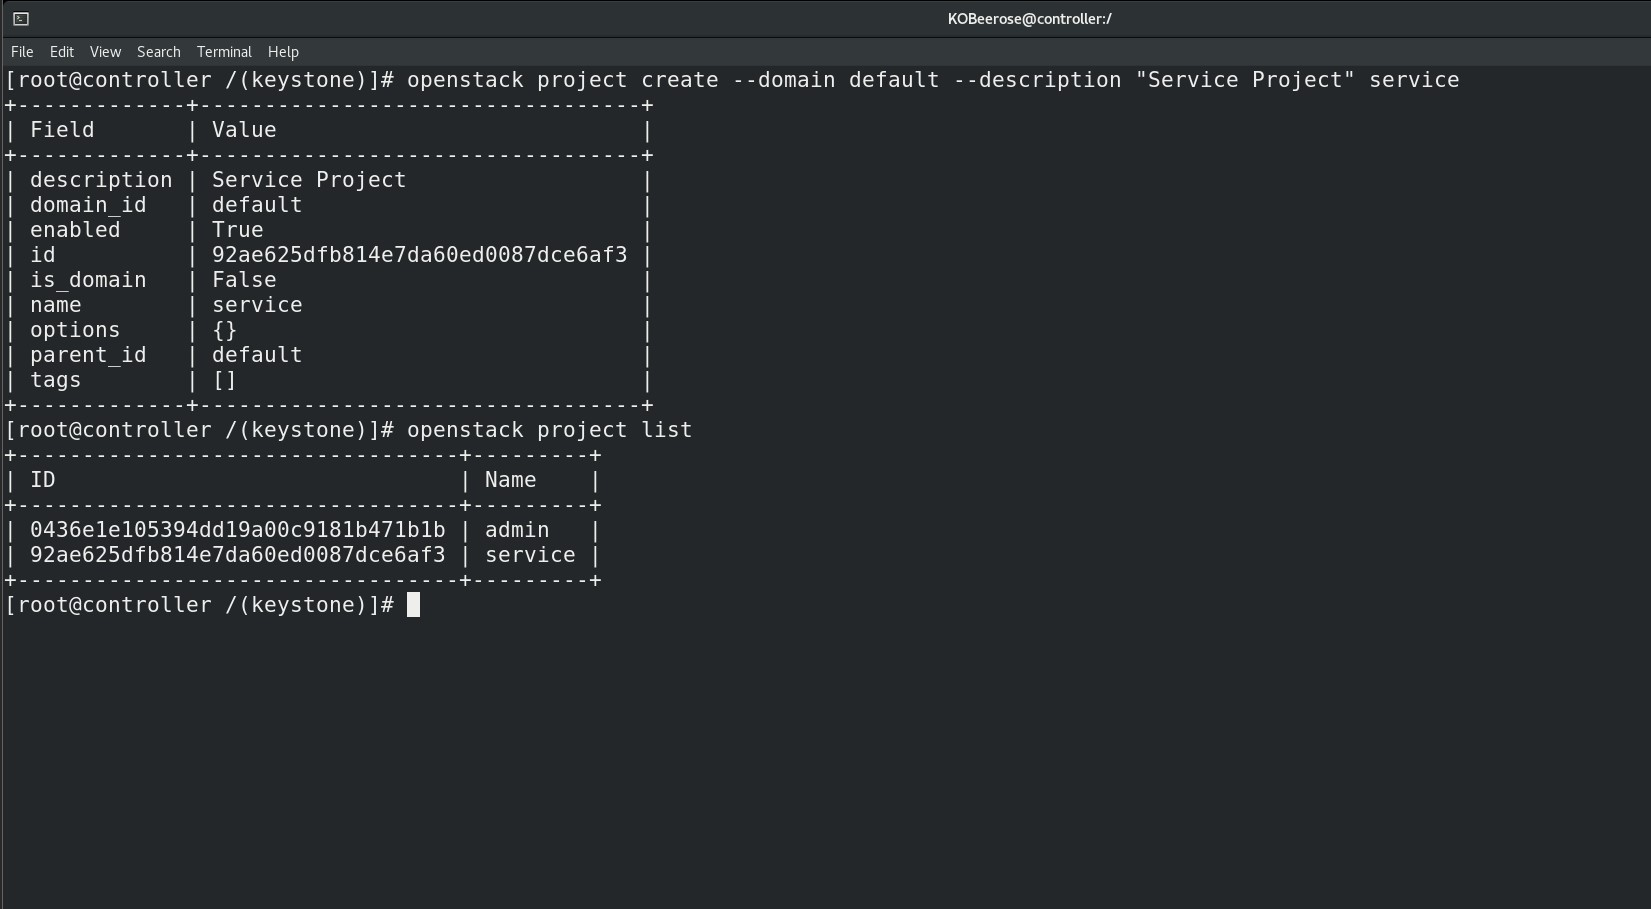
\includegraphics[width=.94\linewidth]{Cloud/Configure Keystone #2/Create Project} 
\end{center} 
\caption{Create Project} 
\end{figure}  \FloatBarrier
\\

\end{spacing}